\documentclass[12pt, letterpaper]{article}

\usepackage{placeins}
\usepackage{appendix}
\usepackage{todonotes}
\usepackage{graphicx}
\usepackage{titling}
\usepackage{xcolor}

% Palatino font for text and math 
\usepackage{mathpazo}
% Bera Mono font for monospace text (code blocks)
\usepackage[scaled]{beramono}
\usepackage[T1]{fontenc}

% Syntax highlighting for Verilog code snippets
\usepackage{listings}
\definecolor{vgreen}{RGB}{104,180,104}
\definecolor{vblue}{RGB}{49,49,255}
\definecolor{vorange}{RGB}{255,143,102}

\lstdefinestyle{verilog-style}
{
    language=Verilog,
    basicstyle=\small\ttfamily,
    keywordstyle=\color{vblue},
    identifierstyle=\color{black},
    commentstyle=\color{vgreen},
    tabsize=2,  % small tab size so code doesn't run off the right-hand-side margin
    literate=*{:}{:}1
}

\title{Lab \# 6 - 8: \textbf{Adding Instruction Decoding to the Datapath}, \textbf{Adding Instruction Memory and Program Counter to Your Computer}, \textbf{Adding Branch Logic to the Datapath to Complete Your Computer}}

% I just copied your name as it appeared in gmail - Tim
\author{Group \# \textbf{14}:\\ Jin Hyeong Kim \and\\ Timothy VanSlyke}


\begin{document}

\begin{titlepage}
	\begin{center}
		{\Large
			\textbf{Northeastern University}\\
			~\\
			Department of Electrical and Computer Engineering\\ 
		}

		\vfill

		{\large
			EECE2323: \textbf{Digital Systems Design Lab}\\
			~\\
			Lecturer: \textbf{Dr. Emad Aboelela}\\
			~\\
			TAs:\\
			\textbf{Ke Chen}\\
			\textbf{Linbin Chen}\\
		}
	
		\vfill

		{\Large \thetitle}\\
	
		\vfill

		{\large \theauthor}\\

		\vfill

		{\large
			Semester: Spring 2018\\
			Date: \today\\
			Lab Session: Tuesday, 1:00PM\\ 
			Lab Location: 9 Hayden Hall, Northeastern University, Boston, MA 02115\\
		}

	\end{center}
\end{titlepage}

\tableofcontents


%%%%%% INTRODUCTION %%%%%%
\newpage
\section{Introduction}
In these experiments, we will investigate the problem of introducing an instruction dispatch system to our existing computer.  We will implement a minimal instruction set architecture (ISA) with a MIPS-inspired encoding and mnemonics.  We will equip our computer with an instruction decoder, a persistent instruction memory component, and facilities for conditional instruction jumps.  The instruction decoder, instruction memory + program counter, and branching facilities will be implemented in Verilog and merged into our existing design.

Our experiments will demonstrate the feasibility of our system by showing hardware testing of manual single-instruction dispatch, and automatic, sequential, multiple-instruction dispatch from instruction memory.  Additionally, we will show that our computer is capable of executing arbitrary programs written in our MIPS-like assembly language.  

%%%%%% DESIGN APPROACH %%%%%%
\newpage
\section{Design Approach}

\subsection{Instruction Set Architecture}
Our ISA encoding follows the conventions of MIPS with R-Type, I-Type, and J-Type instruction categories.  Since our computer cannot correctly implement the MIPS computer model, our encoding diverges slightly from the traditional MIPS encoding. 

We choose to encode our instructions in a 16-bit double word.  Since our computer has only 4 registers, all encodings of source and destination registers use 2-bit slices of the 16-bit encoding.  Our limited instruction set allows us to encode all ALU op-codes in only 4-bit slices.  The R-Type instruction encoding concatenates (from MSB to LSB) a 4-bit op-code followed by three 2-bit register encodings.  The first encoded register is the first source register, the second encoded register is the second source register, and the last register is the destination register in which the ALU output is stored.  The last six unused padding bits are zeroed in all R-Type encodings.
\begin{figure}[h]
\centering
\begin{tabular}{|r|r|r|r|r|}
\hline
Opcode & RS     & RT     & RD     & Padding \\
\hline
4 Bits & 2 Bits & 2 Bits & 2 Bits & 6 Bits \\ 
\hline
\end{tabular}
\caption{Encoding of an R-Type instruction for our ISA.}
\end{figure}

Both I-Type and J-Type encodings are identical in their format.  A 4-bit opcode precedes the source and destination register encodings.  The last 8 bits are used to encode a single-word immediate which is interpreted as an 8-bit two's complement signed integer.  For I-Type instructions, this immediate is a numeric literal used by the ALU to perform its computation, while for J-Type instructions, the immediate is the signed distance to the jump destination.
\begin{figure}[h]
\centering
\begin{tabular}{|r|r|r|r|}
\hline
Opcode & RS     & RT     & Immediate \\ 
\hline
4 Bits & 2 Bits & 2 Bits & 8 Bits \\
\hline
\end{tabular}
\caption{Encoding of an I-Type instruction for our ISA.}
\end{figure}

\subsection{Implementing the ISA in Hardware}
Our instruction dispatch 



\begin{figure}[h]
\centering
\begin{tabular}{|r|r|r|r|}
\hline
Opcode & RS     & RT     & Immediate \\ 
\hline
4 Bits & 2 Bits & 2 Bits & 8 Bits \\ 
\hline
\end{tabular}
\caption{Encoding of a J-Type instruction for our ISA.}
\end{figure}




%%%%%% RESULTS AND ANALYSIS %%%%%%
\newpage
\section{Results and Analysis}

\subsection{Design Simulation}

\subsection{Hardware Testing}
\FloatBarrier

\begin{figure}[h]
\centering
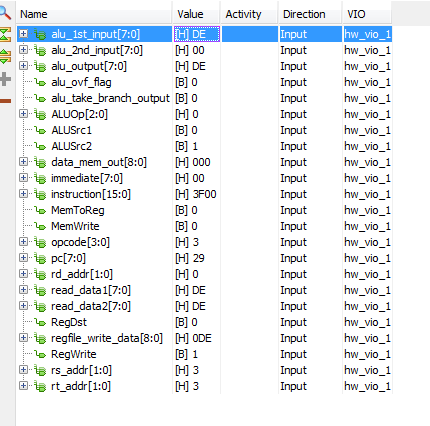
\includegraphics[width=0.8\linewidth]{images/lab8-hardware-test-1.png}
\caption{Hardware VIO testing results.}
\end{figure}

\begin{figure}[h]
\centering
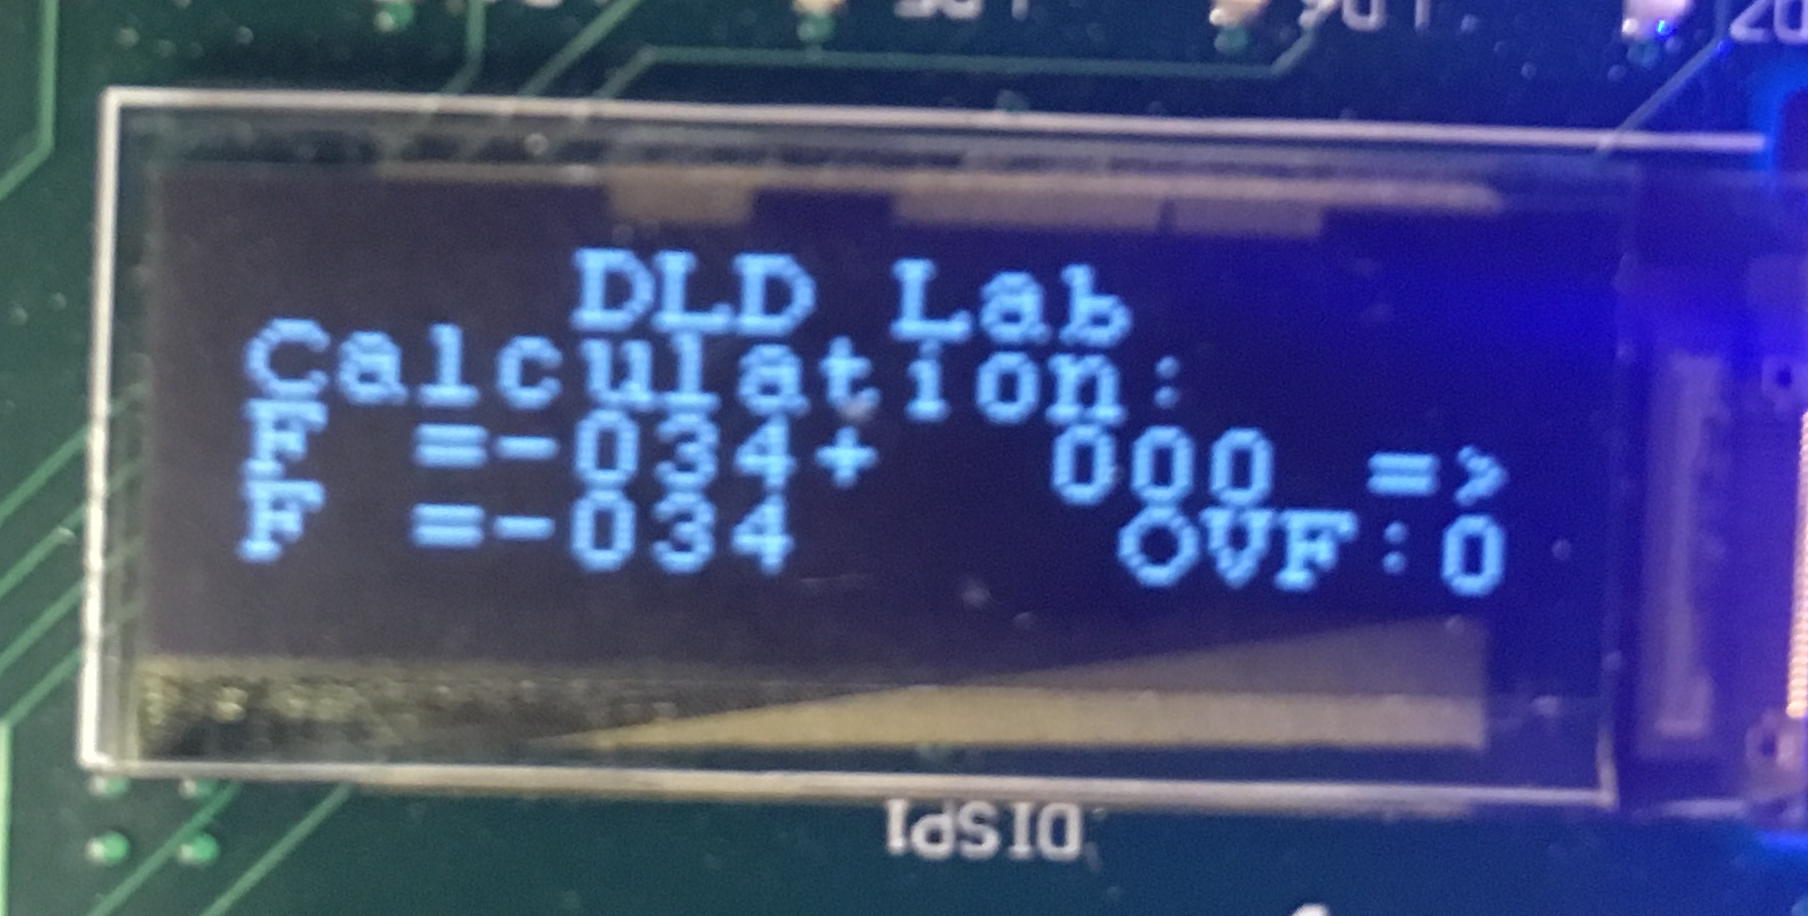
\includegraphics[width=0.8\linewidth]{images/lab8-hardware-test-2.png}
\caption{Hardware test showing software multiply implementation giving the result -34.}
\end{figure}


%%%%%% CONCLUSIONS %%%%%%
\FloatBarrier\newpage
\section{Conclusions}


%%%%%% APPENDICES %%%%%%
\newpage
\appendix
% explicit 'Appendix' in title before appendix sections
\appendixpage
% explicit 'Appendix' in table of contents
\addappheadtotoc 


\end{document}
